\documentclass[../mathNotesPreamble]{subfiles}

\providecommand{\relscalefact}{1.4}
\begin{document}
\relscale{\relscalefact}
  \section{5.1: Angles}
  \begin{defn*}
    A \textbf{ray} consists of one point on a line, and all points extending in one direction from that point. The following is ray $\overrightarrow{EF}$:
    \begin{center}
      \begin{tikzpicture}[
        ->, draw=lander_blue, line width=1pt,
        every node/.style={circle, minimum size=5pt, inner sep=1pt, fill=lander_blue, text=black, draw=lander_blue}]
        \draw (0,0) -- (4,0.5)
          node[pos=0, label=below: $E$] {}
          node[pos=0.8, label=below: $F$, fill=white] {}; 
      \end{tikzpicture}
    \end{center}
    
    An \textbf{angle} is the union of two rays having a common endpoint. The endpoint is called the \textbf{vertex} of the angle. Angles can be named using a point on each ray and the vertex. The following is $\angle DEF$:
    \begin{center}
      \hspace*{\stretch{1}}%
      \begin{minipage}{0.4\linewidth}
        \centering 
        \begin{tikzpicture}[
          ->, draw=lander_blue, line width=1pt,
          every node/.style={circle, minimum size=5pt, inner sep=1pt, fill=lander_blue, text=black, draw=lander_blue}]
          \draw (0,0) -- (1, 2)
            node[pos=0.75, label=left: $D$, fill=white] {};
          \draw (0,0) -- (4,0.5)
            node[pos=0, label=left: $E$, label=below right: Vertex] {}
            node[pos=0.8, label=below: $F$, draw=lander_blue, fill=white] {}; 
        \end{tikzpicture}
      \end{minipage} \hspace*{\stretch{1}}%
      \begin{minipage}{0.4\linewidth}
        \begin{tikzpicture}[
          ->, draw=lander_blue, line width=1pt,
%          every node/.style={circle, minimum size=5pt, inner sep=1pt, fill=lander_blue, text=black, draw=lander_blue}
          ]
          % coordinates formed by transforming EF to x-axis
          \coordinate (D) at (1.2403, 1.8605);
          \coordinate (E) at (0,0);
          \coordinate (F) at (4.0311,0);
          \draw (E) -- (D)
            node[pos=0.75, label=left: Terminal side] {};
          \draw (E) -- (F)
            node[pos=0, label=left: Vertex] {}
            node[pos=0.5, label=below: Initial side] {}; 
          
          \draw[black,->] ($(E)+(1,0)$) arc [start angle=0, end angle=56.3099, radius=1cm];
%          \tkzFillAngle[fill= ClemsonOrange!90,size=1.0cm, opacity=0.95](C,B,A)
%          \tkzLabelAngle[pos = 0.75, draw=none, fill=none](F,E,D){$\theta$}
        \end{tikzpicture}
      \end{minipage}
      \hspace*{\stretch{1}}%
    \end{center}
    When we create an angle, we fix one ray, called the \textbf{initial side}, and rotate the \textbf{terminal side} about the vertex.
    
    An angle drawn on the $xy$-plane is said to be in \textbf{standard position} if its vertex is located at the origin, and the initial side extends along the $x$-axis:
    \begin{center}
      \begin{tikzpicture}[
        myLine/.style={line width=1.5pt, lander_blue, <->},
        line cap=round, line join=round]
        \begin{groupplot}[
          group style={group size=2 by 1,horizontal sep=20mm},
          axis equal,
          xmin=-1.25, xmax=1.25,
          ymin=-1.25, ymax=1.25,
          xmajorticks=false,
          ymajorticks=false,
          height=0.775*\axisdefaultheight,
          ]
          \nextgroupplot
            \draw[myLine] (-0.866,0.5) -- (0,0) -- (1,0);
            \draw[black,->] (0.5,0) arc [start angle=0, end angle=150, radius=0.5]
              node[pos=0.5, above right, inner sep=0pt] {$150^\circ$};
          \nextgroupplot
            \draw[myLine] (0.707,-0.707) -- (0,0) -- (1,0);
            \draw[black,->] (0.5,0) arc [start angle=0, end angle=-45, radius=0.5]
              node[pos=0.05, below right, inner sep=5pt] {$-45^\circ$};
        \end{groupplot}
      \end{tikzpicture}
    \end{center}
    A \textbf{positive angle} rotates in the counterclockwise direction. A \textbf{negative angle} rotates in the clockwise direction. A full circle rotation is defined to be $360^\circ$.
  \end{defn*}
  \pagebreak

  \begin{ex*}
    Sketch the following angles in standard position:
    \begin{center}
      \begin{tikzpicture}[
        myLine/.style={line width=1.5pt, lander_blue, <->},
        line cap=round, line join=round]
        \begin{groupplot}[
          group style={group size=2 by 3,horizontal sep=30mm, vertical sep=14mm},
          axis equal,
          xmin=-1.25, xmax=1.25,
          ymin=-1.25, ymax=1.25,
          xmajorticks=false,
          ymajorticks=false,
          height=0.9*\axisdefaultheight,
          xlabel=, ylabel=,
          ]
          \nextgroupplot[title=$0^{\mathrlap{\circ}}$]
          \nextgroupplot[title=$30^{\mathrlap{\circ}}$]
          \nextgroupplot[title=$90^{\mathrlap{\circ}}$]
          \nextgroupplot[title=$45^{\mathrlap{\circ}}$]
          \nextgroupplot[title=$135^{\mathrlap{\circ}}$]
          \nextgroupplot[title=$-60^{\mathrlap{\circ}}$]
        \end{groupplot}
      \end{tikzpicture}
    \end{center}
  \end{ex*}
  \pagebreak

  \begin{defn*}
    A \textbf{radian} is the measure of a central angle corresponding to an arc equal in length to the radius of that circle. Since the circumference of a circle is $C=2\pi r$, there are $2\pi$ radians in a full circle. This gives us
      \[2\pi=360^\circ\]
    or, equivalently,
      \[\pi=180^\circ\]
  \end{defn*}

  \begin{ex*}
    Convert the following angles to radians:
    \begin{extasks}[after-item-skip=\stretch{1}](2)
      \task $225^\circ$
      \task $270^\circ$
      \task $-135^\circ$
      \task $-45^\circ$
    \end{extasks}
    \vspace*{\stretch{1}}
  \end{ex*}
  
    \begin{ex*}
    Convert the following angles to degrees:
    \begin{extasks}[after-item-skip=\stretch{1}](2)
      \task $4\pi$
      \task $-\dfrac{\pi}{2}$
      \task $\dfrac{\pi}{12}$
      \task $-\dfrac{5\pi}{4}$
    \end{extasks}
    \vspace*{\stretch{1}}
  \end{ex*}
  \pagebreak

  \begin{ex*} 
    The following circle contains certain angles of interest. Find the angles of each in both degrees and radians:
    \vspace*{2\baselineskip}

  \newcommand{\lCol}{gray!90}
    \begin{center}
      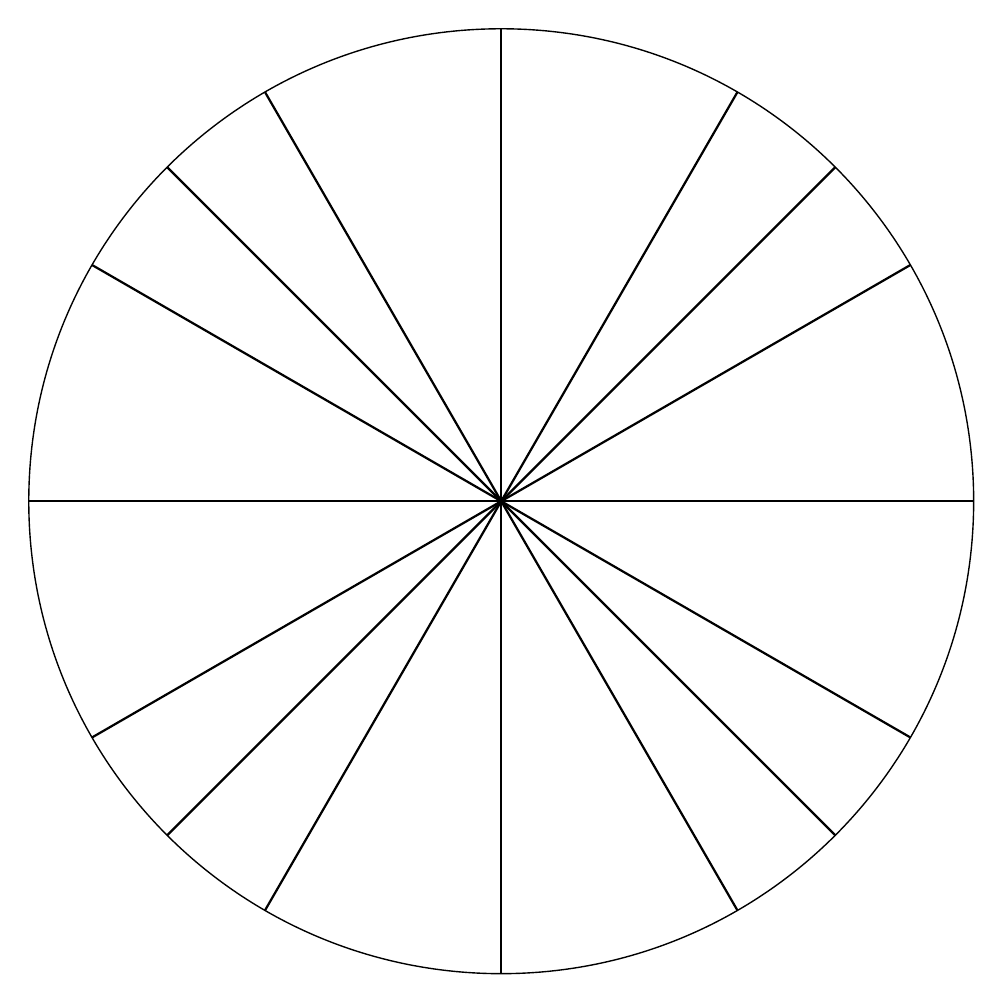
\begin{tikzpicture}[scale=6, line width=0.8pt]
        \draw[line width=0.5pt] (0,0) circle(1);
        \foreach \x in {0,30,...,360} 
            \draw[\lCol] (0cm,0cm) -- (\x:1);

        \foreach \x in {45,135,225,315} 
            \draw[\lCol] (0cm,0cm) -- (\x:1);
      \end{tikzpicture}
    \end{center}
  \end{ex*}
  \pagebreak

  \begin{defn*}
    \textbf{Coterminal angles} are two angles in standard position that have the same terminal side.
    
%    An angle's \textbf{reference angle} is the size of the smallest is the size of the smallest acute angle, $t'$, formed by the terminal side of the angle $t$ and the horizontal axis.
  \end{defn*}
  \begin{ex*}
    Find a coterminal angle for each of the following:
    \begin{extasks}[after-item-skip=\stretch{1}](2)
      \task $400^\circ$
      \task $-30^\circ$
      \task $1655^\circ$
      \task $-500^\circ$
      \task $7\pi$
      \task $\dfrac{-5\pi}{6}$
      \task $\dfrac{21\pi}{4}$
      \task $-\dfrac{17\pi}{3}$
    \end{extasks}
    \vspace*{\stretch{1}}
  \end{ex*}

  \pagebreak
\end{document}
